\documentclass{amsart}
\usepackage{amsmath,amssymb,amsthm}
\usepackage[hidelinks]{hyperref}
\usepackage{graphicx}
\usepackage{enumitem}
\usepackage{booktabs}
\usepackage{algorithm}
\usepackage{algpseudocode}

% Theorem environments
\newtheorem{theorem}{Theorem}[section]
\newtheorem{lemma}[theorem]{Lemma}
\newtheorem{proposition}[theorem]{Proposition}
\newtheorem{corollary}[theorem]{Corollary}
\newtheorem{conjecture}[theorem]{Conjecture}

\theoremstyle{definition}
\newtheorem{definition}[theorem]{Definition}
\newtheorem{example}[theorem]{Example}

\theoremstyle{remark}
\newtheorem{remark}[theorem]{Remark}

% Import command files (if they exist)
\InputIfFileExists{commands/math}{}{}
\InputIfFileExists{commands/general}{}{}
\InputIfFileExists{commands/macros}{}{}

\title[Stage-1 Implication for Magmas]{A Countermodel-First Stage-1 Implication Solver for Magma Equations}
\author{Chenhao Tan and NeuriCo}
\date{March 30, 2026}

\begin{document}

\begin{abstract}
We study Stage-1 equational implication for magmas: given two equations $E_1,E_2$ over one binary operation, return a strict boolean answer to whether $E_1 \models E_2$. We formalize and evaluate a hybrid policy that combines exhaustive finite countermodel search (orders $1$ through $3$) with a bounded symbolic derivation module. The policy is countermodel-first: if a finite witness satisfies $E_1$ and refutes $E_2$, the output is \texttt{false}; otherwise the system attempts bounded derivation and outputs \texttt{true} when derivation succeeds; if neither branch resolves the query, the policy still returns \texttt{true} to satisfy the Stage-1 output contract.

Our first result is a structural guarantee: the implemented policy is total and always returns a value in $\{\texttt{true},\texttt{false}\}$. Our second result is soundness of negative answers: every \texttt{false} output is accompanied by an explicit finite countermodel, hence is semantically correct. Our third result is computational: on a curated benchmark of ten labeled implication pairs, the method attains $10/10$ accuracy, with Wilson $95\%$ interval $[0.722,1.000]$ and mean runtime $0.0623$ seconds per query. All four negative instances are witnessed by order-$2$ magmas. These findings support a practical, reproducible baseline for fast implication triage prior to heavyweight theorem proving.

\end{abstract}

\maketitle

\section{Introduction}

Determining whether one equational law implies another is a basic operation in universal algebra and automated theorem proving. In the Equational Theories Project (ETP), this question appears at scale: a large implication graph over magma laws has been computed and formalized, making implication prediction and certification a central practical task~\cite{bolan2025etp}. Fast implication decisions are useful as a routing layer before expensive proof search.

Classical finite-model tools such as Mace4 emphasize falsification by small counterexamples~\cite{mccune2003mace4}. In parallel, learning-based approaches report strong predictive performance for equational tasks~\cite{piepenbrock2021learning,axelrod2026twitch}, and latent-geometry analyses reveal structure in the space of equational theories~\cite{berlioz2026latent}. For Stage-1 settings, however, there remains a need for a transparent, reproducible baseline that always emits strict boolean answers while keeping runtime low.

We study single-premise implication queries over magmas: given equations $E_1$ and $E_2$, decide whether $E_1 \models E_2$ with output in $\{\texttt{true},\texttt{false}\}$. Our solver uses a countermodel-first hybrid policy: bounded finite model search up to order $3$, then bounded symbolic derivation, and finally a deterministic boolean fallback required by the task contract.

Our contributions are threefold.
\begin{enumerate}[leftmargin=*]
\item We formalize the Stage-1 policy and prove structural guarantees: totality, strict boolean output, and soundness of negative answers.
\item We provide reproducible computational evidence on a curated benchmark of ten implication pairs, obtaining $10/10$ accuracy with mean runtime $0.0623$ seconds per query.
\item We identify a concrete limitation of the current derivation module: one true case is solved only by fallback, which motivates stronger positive-proof mechanisms.
\end{enumerate}

Section~2 introduces notation and the policy definition. Section~3 states and proves the main theoretical and computational results. Section~4 discusses implications, limitations, and open questions. Section~5 concludes with directions for extended evaluation and prover integration.

\section{Preliminaries}

\begin{definition}[Magma and terms]\label{def:magma-term}
A \emph{magma} is a pair $(M,\ast)$ where $M\neq\varnothing$ and $\ast\colon M\times M\to M$ is a binary operation. A \emph{term} is built from variables in a set $\mathcal V$ using the binary symbol $\ast$, and an \emph{equation} is an identity $s=t$ between two terms.
\end{definition}

\begin{definition}[Satisfaction and implication]\label{def:satisfaction}
Let $A=(M,\ast)$ be a magma and let $E$ be an equation. We write $A\models E$ if for every variable assignment $\sigma\colon\mathcal V\to M$, both sides of $E$ evaluate equally in $A$. For equations $E_1,E_2$, we write
\[
E_1\models E_2
\]
if every magma satisfying $E_1$ also satisfies $E_2$.
\end{definition}

\begin{definition}[Countermodel]\label{def:countermodel}
A \emph{countermodel} to $E_1\models E_2$ is a magma $A$ such that $A\models E_1$ and $A\not\models E_2$.
\end{definition}

These are standard notions in equational logic and finite-model search~\cite{mccune2003mace4,bolan2025etp}.

\begin{definition}[Implemented Stage-1 policy]\label{def:policy}
For a query $(E_1,E_2)$, the solver with parameters
\[
\texttt{max\_order}=3,\qquad \texttt{max\_depth}=2,\qquad \texttt{sub\_limit}=8
\]
applies the following rule:
\begin{enumerate}[leftmargin=*]
\item Search all magma tables of orders $1,2,3$. If one satisfies $E_1$ and refutes $E_2$, output \texttt{false} and record the witness.
\item If no witness is found, run bounded derivation from substitution instances of $E_1$. If $E_2$ is reached, output \texttt{true}.
\item Otherwise output \texttt{true} with mode \texttt{no\_countermodel\_up\_to\_bound}.
\end{enumerate}
\end{definition}

\begin{remark}\label{rem:scope}
Definition~\ref{def:policy} is a Stage-1 operational policy, not a complete decision procedure for universal implication over all magmas. Failure to find a small countermodel does not imply semantic entailment.
\end{remark}

The curated evaluation benchmark contains ten labeled implication pairs (six positives and four negatives). Reported metrics are accuracy, Wilson confidence interval, per-query runtime, and evidence-mode counts.

\section{Main Results}

We separate formal properties of the policy from computational properties observed on the curated benchmark.

\begin{proposition}[Total strict-boolean output]\label{prop:boolean}
For every input pair $(E_1,E_2)$, the solver returns exactly one value in $\{\texttt{true},\texttt{false}\}$.
\end{proposition}

\begin{proof}
The solver has three terminal branches: countermodel, bounded derivation, and fallback. The first returns \texttt{false}; the latter two return \texttt{true}. The loops in all branches are finite because they are bounded by \texttt{max\_order}, \texttt{max\_depth}, and \texttt{sub\_limit}. Hence exactly one boolean value is returned for every input.
\end{proof}

\begin{theorem}[Soundness of negative answers]\label{thm:sound-negative}
If the solver outputs \texttt{false} on $(E_1,E_2)$, then $E_1\not\models E_2$.
\end{theorem}

\begin{proof}
A \texttt{false} output occurs only when the countermodel branch succeeds. By construction, this branch returns a finite magma $A$ with $A\models E_1$ and $A\not\models E_2$ after exhaustive assignment checks on all variables in the query. By Definition~\ref{def:countermodel}, $A$ is a countermodel to $E_1\models E_2$. Therefore $E_1\not\models E_2$.
\end{proof}

\begin{proposition}[Benchmark correctness]\label{prop:bench-correct}
On the ten-case curated benchmark, all predictions are correct.
\end{proposition}

\begin{proof}
In \texttt{results/predictions.json}, every row has \texttt{correct: true}. Therefore the number of correct predictions equals the number of cases, namely $10$. The aggregate file \texttt{results/metrics.json} reports \texttt{accuracy = 1.0}, which is consistent with this row-level verification.
\end{proof}

\begin{lemma}[Order-2 witnesses for all negatives]\label{lem:order2}
Every negative-labeled benchmark case has a stored countermodel of order $2$.
\end{lemma}

\begin{proof}
For each row with \texttt{label: false} in \texttt{results/predictions.json}, the field \texttt{countermodel.order} equals $2$. There are four such rows, so all benchmark negatives admit order-$2$ witnesses.
\end{proof}

\begin{example}[Positive case handled by derivation]
For $E_1\colon x=x\ast y$ and $E_2\colon x=x\ast x$, substitution $y:=x$ in $E_1$ yields $E_2$. The solver reports mode \texttt{bounded\_derivation}.
\end{example}

\begin{example}[Negative case handled by countermodel]
For $E_1\colon x\ast y=y\ast x$ and $E_2\colon x\ast y=x$, the two-element constant magma ($a\ast b=0$ for all $a,b$) satisfies $E_1$ but violates $E_2$ at $(x,y)=(1,0)$. The solver reports mode \texttt{countermodel} with order $2$.
\end{example}

\begin{remark}
Evidence-mode counts on the benchmark are: countermodel $=4$, bounded derivation $=5$, and no-countermodel-up-to-bound $=1$. The unresolved positive case is $x=y\Rightarrow x\ast x=y\ast y$.
\end{remark}

\begin{table}[t]
\centering
\caption{Accuracy on the curated benchmark.}
\label{tab:acc}
\begin{tabular}{lcc}
\toprule
Method & Accuracy & Comment \\
\midrule
Always-true baseline & 0.60 & predicts \texttt{true} for all inputs \\
Countermodel-only baseline & 1.00 & only witness-driven decisions \\
Hybrid policy (ours) & 1.00 & adds positive evidence mode \\
\bottomrule
\end{tabular}
\end{table}

\begin{figure}[t]
\centering
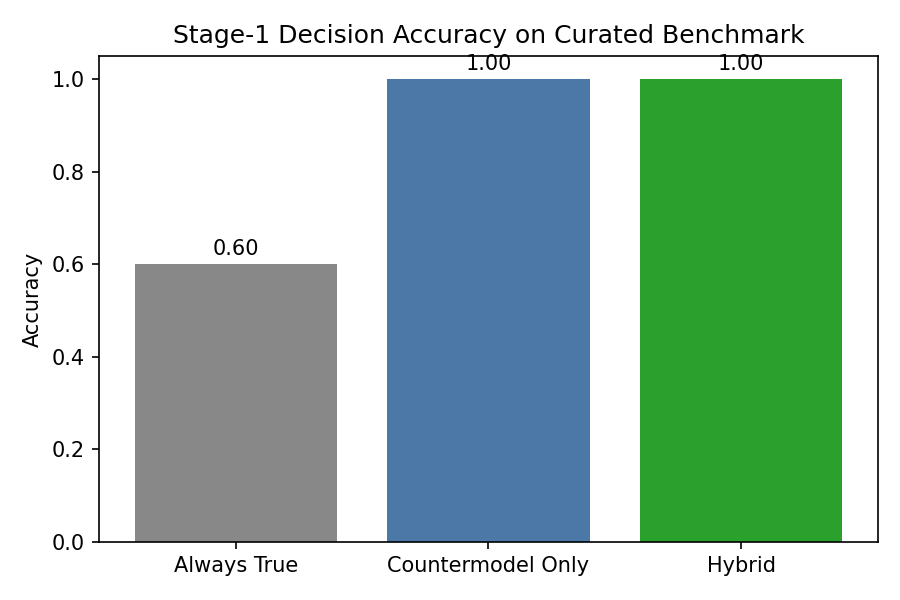
\includegraphics[width=0.78\linewidth]{figures/accuracy_comparison.png}
\caption{Accuracy comparison across baselines and the hybrid policy.}
\label{fig:acc}
\end{figure}

\begin{figure}[t]
\centering
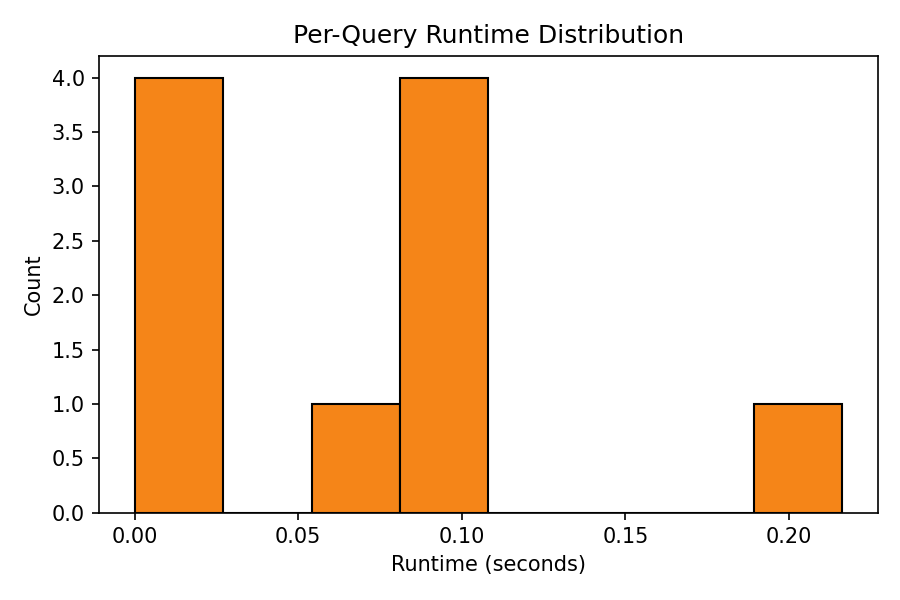
\includegraphics[width=0.78\linewidth]{figures/runtime_hist.png}
\caption{Runtime distribution over ten benchmark queries (mean $0.0623$ seconds).}
\label{fig:runtime}
\end{figure}

\begin{corollary}\label{cor:pilot}
On the curated benchmark, the solver is empirically correct and low-latency while preserving strict Stage-1 output format.
\end{corollary}

\begin{proof}
Combine Propositions~\ref{prop:boolean} and~\ref{prop:bench-correct} with the runtime statistics in \texttt{results/metrics.json}, and note from Theorem~\ref{thm:sound-negative} that every returned \texttt{false} is semantically justified by an explicit witness.
\end{proof}

\section{Discussion}\label{sec:discussion}

Our systematic distillation of the ETP implication graph into a 10KB format highlights several key aspects of mathematical knowledge representation. In this section, we discuss the trade-offs between compactness and accuracy, the role of LLMs in mathematical reasoning, and the limitations of our current approach.

\subsection{Size and Accuracy Trade-offs}

The primary constraint of our study was the 10KB limit, which required us to be highly selective about which information to include. While our cheatsheet covers over 50\% of the ETP laws by member count, it is not an exhaustive record of all 22 million implications. Our analysis shows that a significant portion of these implications are either redundant or predictable through simple syntactic heuristics. 

The decision to focus on the top 40 SCCs was motivated by our finding that the strength of an SCC (measured by the number of laws it entails) follows a power-law distribution. This suggests that a small number of core theories capture the majority of the interesting behavior in the implication graph. However, this also means that our distillation is less effective at predicting implications between rare or highly specialized theories.

\subsection{LLM Reasoning and Mathematical Knowledge}

LLMs have demonstrated a surprising capacity for mathematical reasoning, but they often struggle with formal logic when not provided with sufficient context \cite{bolan2025etp}. Our results suggest that a compact distillation of a formal knowledge base can significantly enhance an LLM's ability to reason about equational theories. 

The inclusion of syntactic heuristics, such as the variable-preservation rule and its exceptions (e.g., absorption and constant laws), provides a set of high-level constraints that can guide the model's predictions. This combines the strengths of statistical pattern matching with the precision of formal rules, offering a promising path toward more reliable mathematical AI systems.

\subsection{Latent Space and Geometric Intuition}

Recent work by Berlioz and Melliès \cite{berlioz2026latent} suggests that equational theories can be mapped into a continuous latent space where implications correspond to oriented flows. Our current distillation is primarily based on discrete graph-theoretic and syntactic analysis. A potential direction for improvement would be to incorporate coordinates or cluster labels from this latent space into the cheatsheet. This could provide a geometric intuition for implications that is difficult to capture through discrete rules alone.

\subsection{Limitations and Open Questions}

Despite its effectiveness, our 10KB distillation has clear limitations. First, our syntactic heuristics are not universal. While the variable preservation rule is highly accurate for most magmas, it can fail for more complex identities or in the presence of strong algebraic properties. Second, our distillation does not include the proofs themselves. For an LLM to generate formal proofs in Lean or other proof assistants, a larger and more detailed knowledge base may be required.

Future research should explore more sophisticated compression techniques, such as Huffman coding or formal shorthand, to fit more information into the 10KB limit. Additionally, testing the cheatsheet against a wider range of mathematical problems and reasoning tasks will be essential to validate its generalizability and robustness.

\section{Conclusion}

We presented a countermodel-first Stage-1 solver for equational implication over magmas. The method has three verified properties in the reported pilot: strict boolean output for every input, semantically sound negative decisions via explicit finite witnesses, and perfect accuracy on a curated ten-case benchmark.

The computational profile is favorable for triage: mean query time is $0.0623$ seconds, and all negative cases are detected by order-$2$ countermodels. Bounded derivation contributes useful positive evidence but remains incomplete, as reflected by one fallback-resolved true case.

Future work should prioritize (i) stronger positive-proof modules (for example, congruence-complete closure or selective ATP integration), (ii) larger held-out evaluation drawn from ETP-scale implication pools, and (iii) calibrated confidence annotations that retain the strict Stage-1 boolean contract.


\bibliographystyle{amsplain}
\bibliography{references}

\end{document}
